\documentclass[AArch64-RaspberryPI-OS-14325283.tex]{subfiles}

\usepackage{tikz}
\usetikzlibrary{positioning}
\usetikzlibrary{arrows.meta}

\begin{document}
\begin{figure}[htpb]
\centering
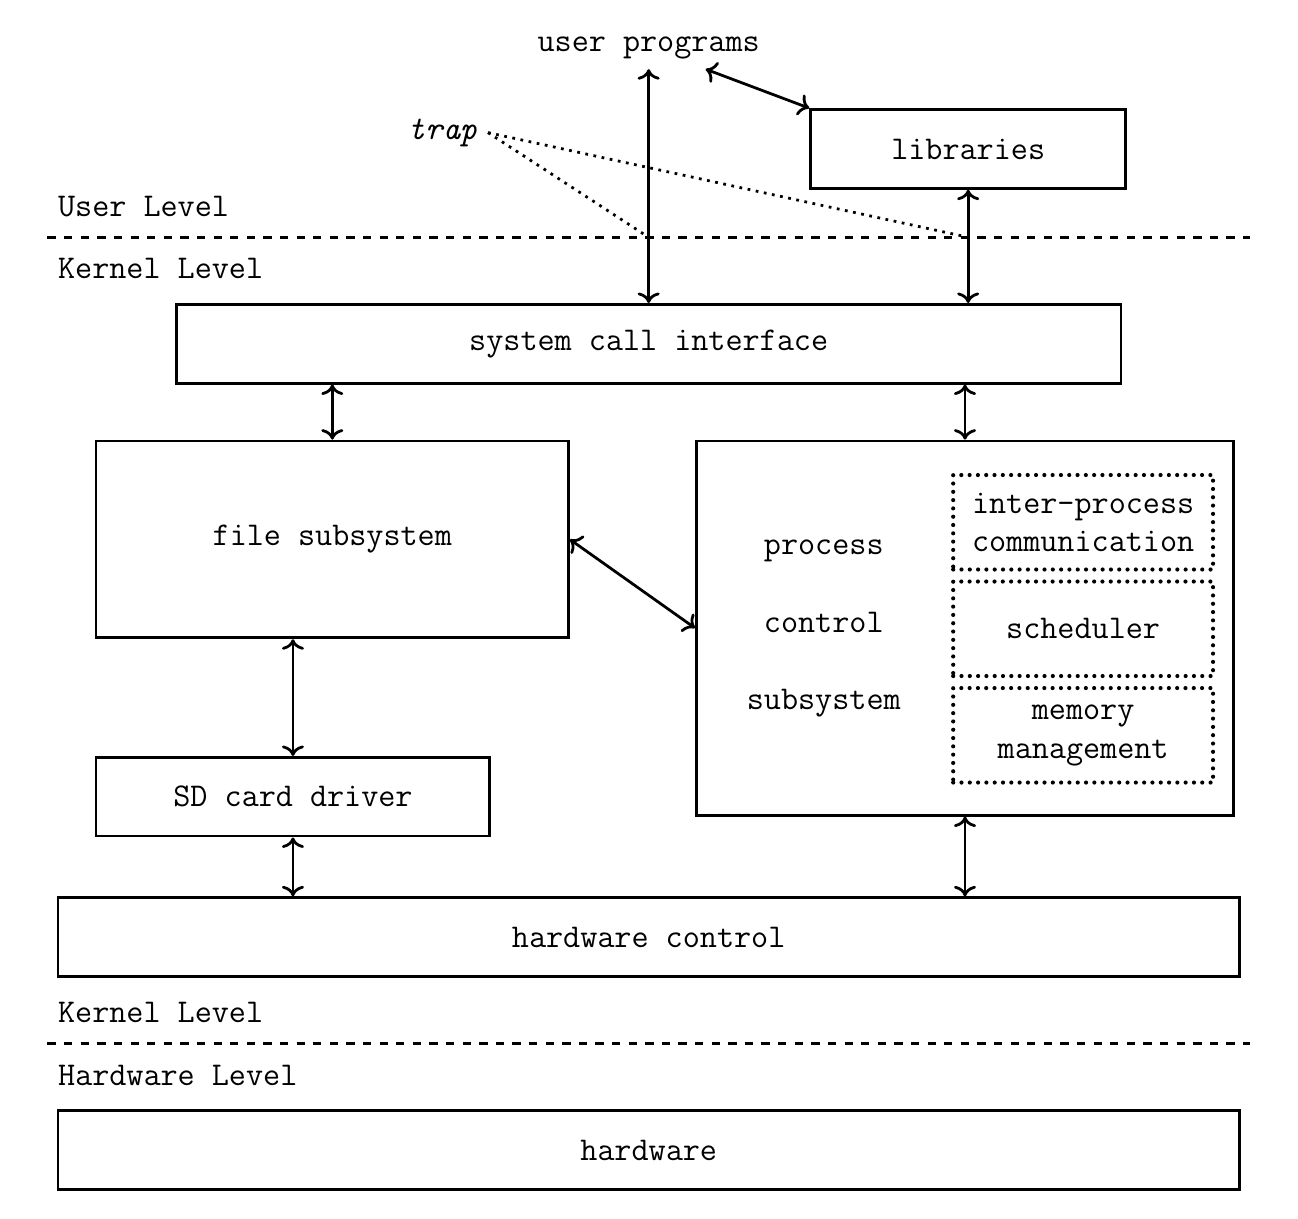
\begin{tikzpicture}[every node/.append style={line width=1pt, font=\bfseries\ttfamily\large},
                    itlabel/.style={font=\ttfamily\large\itshape},
                    box/.style={rectangle, draw, minimum size=1cm, align=center},
                    widebox/.style={box, minimum width=12cm},
                    fullwidthbox/.style={box, minimum width=15cm},
                    dotbox/.style={box, line width=1.5pt, line cap=round, dash pattern=on 0pt off 2\pgflinewidth},
                    every path/.append style={line width=1pt},
                    node distance=7mm]
    \node [] (usrprogs) {user programs};
    \node [box, minimum width=4cm, below right=of usrprogs] (libs) {libraries};
    \node [itlabel, below left=of usrprogs] (trap) {trap};

    % User/kernel level line
    \node [below=2cm of usrprogs] (usr_krn_mid) {};
    \node [left=75mm of usr_krn_mid, label=above right:{User Level}, label=below right:{Kernel Level}] (usr_krn_l) {};
    \node [right=75mm of usr_krn_mid] (usr_krn_r) {};

    \node [widebox, below=of usr_krn_mid] (syscalls) {system call interface};

    \node [box, minimum width=6cm, minimum height=25mm, below=of syscalls.south west, xshift=2cm] (fs) {file subsystem};
    \node [matrix, minimum width=3cm, minimum height=45mm, draw=black, below=of syscalls.south east, xshift=-2cm] (pcs matrix) {
        \node [align=center, minimum height=45mm] (pcs_label) {process\\\\control\\\\subsystem};
        & \node{\tikz[node distance=1mm]{
            \node [dotbox, minimum width=33mm, minimum height=12mm] (ipc) {inter-process\\communication};
            \node [dotbox, minimum width=33mm, minimum height=12mm, below=of ipc] (sched) {scheduler};
            \node [dotbox, minimum width=33mm, minimum height=12mm, below=of sched] (mem) {memory\\management};
        }}; \\
    };

    \node [box, minimum width=5cm, below=2cm of fs.south west, anchor=west] (sd) {SD card driver};

    \node [fullwidthbox, below=65mm of syscalls] (hw_interface) {hardware control};

    % Kernel/Hardware level line
    \node [below=of hw_interface] (krn_hw_mid) {};
    \node [left=75mm of krn_hw_mid, label=above right:{Kernel Level}, label=below right:{Hardware Level}] (krn_hw_l) {};
    \node [right=75mm of krn_hw_mid] (krn_hw_r) {};

    \node [fullwidthbox, below=of krn_hw_mid] (hw) {hardware};

    % Draw the dashed lines
    \draw [dashed] (usr_krn_l)  -- (usr_krn_r);
    \draw [dashed] (krn_hw_l) -- (krn_hw_r);
    % Draw the dotted lines
    \draw [dotted] (trap.east)    -- (usrprogs.south|-usr_krn_mid);
    \draw [dotted] (trap.east)    -- (libs.south|-usr_krn_mid);
    % Draw the arrows
    \draw [<->] (usrprogs)                          -- (syscalls);
    \draw [<->] (usrprogs)                          -- (libs.north west);
    \draw [<->] (libs.south)                        -- (libs.south|-syscalls.north);
    \draw [<->] (fs.north|-syscalls.south)          -- (fs.north);
    \draw [<->] (pcs matrix.north|-syscalls.south)  -- (pcs matrix.north);
    \draw [<->] (fs.east)                           -- (pcs matrix.west);
    \draw [<->] (sd.north|-fs.south)                -- (sd.north);
    \draw [<->] (sd.south)                          -- (sd.south|-hw_interface.north);
    \draw [<->] (pcs matrix.south)                  -- (pcs matrix.south|-hw_interface.north);
\end{tikzpicture}
\caption{A diagram of how the components of the operating system will interact
with each other. Inspired by a diagram from a book on
Unix (Figure~2.1 from~\cite{design-of-unix-os}). The versions of this diagram
which are available online are low-resolution, so the version provided here is
in a vector format, and this document's source code is available
online~\cite{this-document}.}
\label{fig:os-block-diagram}
\end{figure}
\end{document}

